\section{Geschichte}
Bereits schon in der Antike, zur Zeit der griechischen Mythologie, wurden die ersten Versuche mit Automaten durchgeführt. Die Automaten der ersten Generation hatten wenig mit Robotern im heutigen Sinne zu tun. Jede Aktion musste vom Menschen abgerufen werden, daher wird hier der Begriff \textit{Automat} anstelle von \textit{Roboter} verwendet.

Der erste sagenhafte Konstrukteur von Maschinen und automatenhaften Gebilden war Daidalos. Es wird erzählt, er habe eine Flugmaschine entworfen, die seinen Sohn Ikarus und ihn selbst vor der Ungnade des Königs Minos retten sollte. 

Aber auch zu Zeiten der Ägypter wurde die Entwicklung von Automaten vorangetrieben. König Ptolemaios von Ägypten förderte im dritten Jahrhundert v. Christus die Automatenentwicklung als Mäzen\footnote{Person oder Institution, die mit Geld oder geldwerten Mitteln bei der Umsetzung eines Vorhabens unterstützt}. Er war auch bekannt dafür, eigene Automaten zu entwickeln. Bei einem Fest zu Ehren Alexanders des Großen soll er eine Statue gebaut haben, die auf ihrem Weg aufgestanden ist und Milch in eine Schale gegossen hat. Aber auch in anderen Kulturen finden sich Erwähnungen solcher (halb-)automatischer Statuen zu Repräsentationszwecken.

Doch nicht nur in der Mythologie finden sich hinweise auf die ersten Automaten. Besonders die Anhänger der Schule von Alexandria (Heron, Philon) bewiesen mit ihren Vorrichtungen nach dem Sanduhrprinzip grundlegende technische Entwicklungen. Dabei dienten ihnen Wasser, Wasserdampf, Winde, Hebel und Flaschenzüge als Energiequellen und Antriebsmittel.

Im 14. Jahrhundert wurde die Weiterentwicklung der Automaten durch die Erfindung der "`Hemmung"' einer Uhr gefördert. Die Abhängigkeit zum Prinzip der Sanduhr wurde aufgelöst. Der Mensch versuchte unter anderem, "`imitatio die"', ein maschinalisiertes Universum nachzubauen. 

In den folgenden Jahrhunderten zielte die technische Entwicklung der Automaten immer mehr auf die perfekte Nachahmung der Natur  ab. Dies perfektionierte vor allem Jacques de Vaucansons. 1738 stellte er einen nahezu lebensgroßen Flötenspieler vor, der zwölf Melodien spielen konnte. Diese wurden naturgetreu durch die entsprechenden Zungen- und Fingerbewegungen erzeugt. Der Höhepunkt seiner Entwicklungen ist die mechanische Ente (siehe Abbildung \ref{f:Ente}). Zum ersten Mal imitiert ein biokinematischer Automat nicht nur äußerlich die Natur, sondern auch innerlich korrekt die biologischen Vorgänge. Es ist nicht ganz klar, wie genau die Verdauung funktioniert, sicher ist jedoch, dass die Ente ihre Nahrung auf natürlichem Wege eingenommen und auch wieder ausgeschieden hat.  

\begin{figure}[H]						
	\centering							
	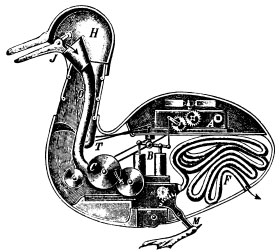
\includegraphics[scale=0.9]{Bilder/Duck_of_Vaucanson.jpg}			
	\caption{Vaucansons Ente}						
	\label{f:Ente}						
\end{figure}
Sodann wurden tatsächliche Automaten nur noch in sehr kleinen Formaten gebaut und diese waren auf Grund der hohen Fertigungskosten ausschließlich für wohlhabende Bürger vorbehalten. Deshalb wendeten sich die Techniker der Entwicklung von Nutzmaschinen zu, die durch die Erfindung von Dampf und Elektrizität als Antriebsmittel deutlich beschleunigt wurden. 

Die Idee Automaten zu bauen, die nützlichere Aufgaben erledigen sollten, kam Anfang des 20. Jahrhunderts. So begann beispielsweise 1951 die Entwicklung ferngesteuerter Geräte zur Interaktion mit radioaktivem Material. 1954 wurde das erste Patent einer Roboterentwicklung durch den Briten C.W. Kenward eingereicht und 1959 der erste kommerzielle Roboter der Firma Planet Corp. vorgestellt. Dieser wurde mechanisch durch Kurvenscheiben und Begrenzungsschalter gesteuert. Ein erster mobiler Roboter (siehe Abbildung \ref{f:shakey}) wurde ca. 1968 am Stanford Research Institute entwickelt. Dieser war erstmals mit Sensoren, wie Kamera oder Tastsensoren ausgestattet.
\begin{figure}[H]						
	\centering							
	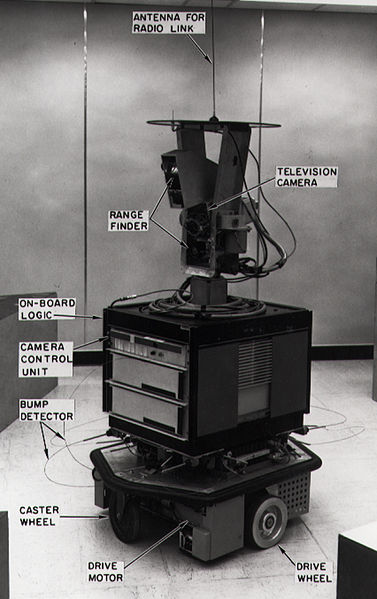
\includegraphics[scale=1]{Bilder/shakey.jpg}			
	\caption{Mobiler Roboter "`Shakey"'}						
	\label{f:shakey}						
\end{figure}
1978 wurde der Roboterarm PUMA\footnote{programmable universal machine for assembly, dt.: Programmierbare Universalmaschine für Montage - Anwendungen} vorgestellt. Er verfügte über einen elektrischen Antrieb und basierte auf Entwürfen von General Motors.
\\
\\
Zeitlich gesehen wird ab 1970 von Robotern gesprochen, da diese immer mehr mit ihrer Umgebung interagierten und nicht mehr "`starr"' ihre Bewegungen ausführten. Der Begriff Roboter oder mobiler Roboter wird im nächsten Abschnitt definiert.
 
